\section{Cloud-native data architecture}
\label{background:cloud-native-data-architecture}
\subsection{Decoupled storage and compute} 
\label{background:cloud-native-data-architecture:decoupled-storage-and-compute}
Traditional data processing systems co-locate storage and compute on the same node, each node being a single server in the cluster, so each node processes only the data it stores locally. This tight coupling, the architectural binding of compute and storage to the same hardware, forces the two layers to scale together, even when demand for each grows at different rates \parencite{dageville2016_snowflake_elastic_data_warehouse}.

Cloud architectures decouple these layers, placing data in object storage and provisioning compute, the on-demand allocation of processing capacity, independently of storage, as Figure~\ref{fig:storage-compute-architectures} illustrates. Object storage is a network-accessible store in which each object is identified by a unique key \parencite{calder2011_windows_azure_storage,mesnier2003_object_based_storage}. It is inexpensive and effectively unbounded in capacity, but offers no query capabilities. The separation allows storage and compute to be scaled, priced, and allocated independently \parencite{pang2024_storage_disaggregated_databases}, and compute can be shut down entirely when idle \parencite{dageville2016_snowflake_elastic_data_warehouse}. Multiple engines, software systems that execute queries against the data, can also read the same underlying data without coordinating through a shared server \parencite{pang2024_storage_disaggregated_databases}. \textcite{dageville2016_snowflake_elastic_data_warehouse} note that this arrangement incurs higher latency and \acrfull{cpu} overhead per request than a node in which compute and storage are tightly coupled. This penalty makes format design critical: formats that minimize the volume of data read per query gain a clear advantage.

\begin{figure}[H]
    \centering
    \subfloat[Coupled storage and compute.\label{fig:coupled-compute}]{%
        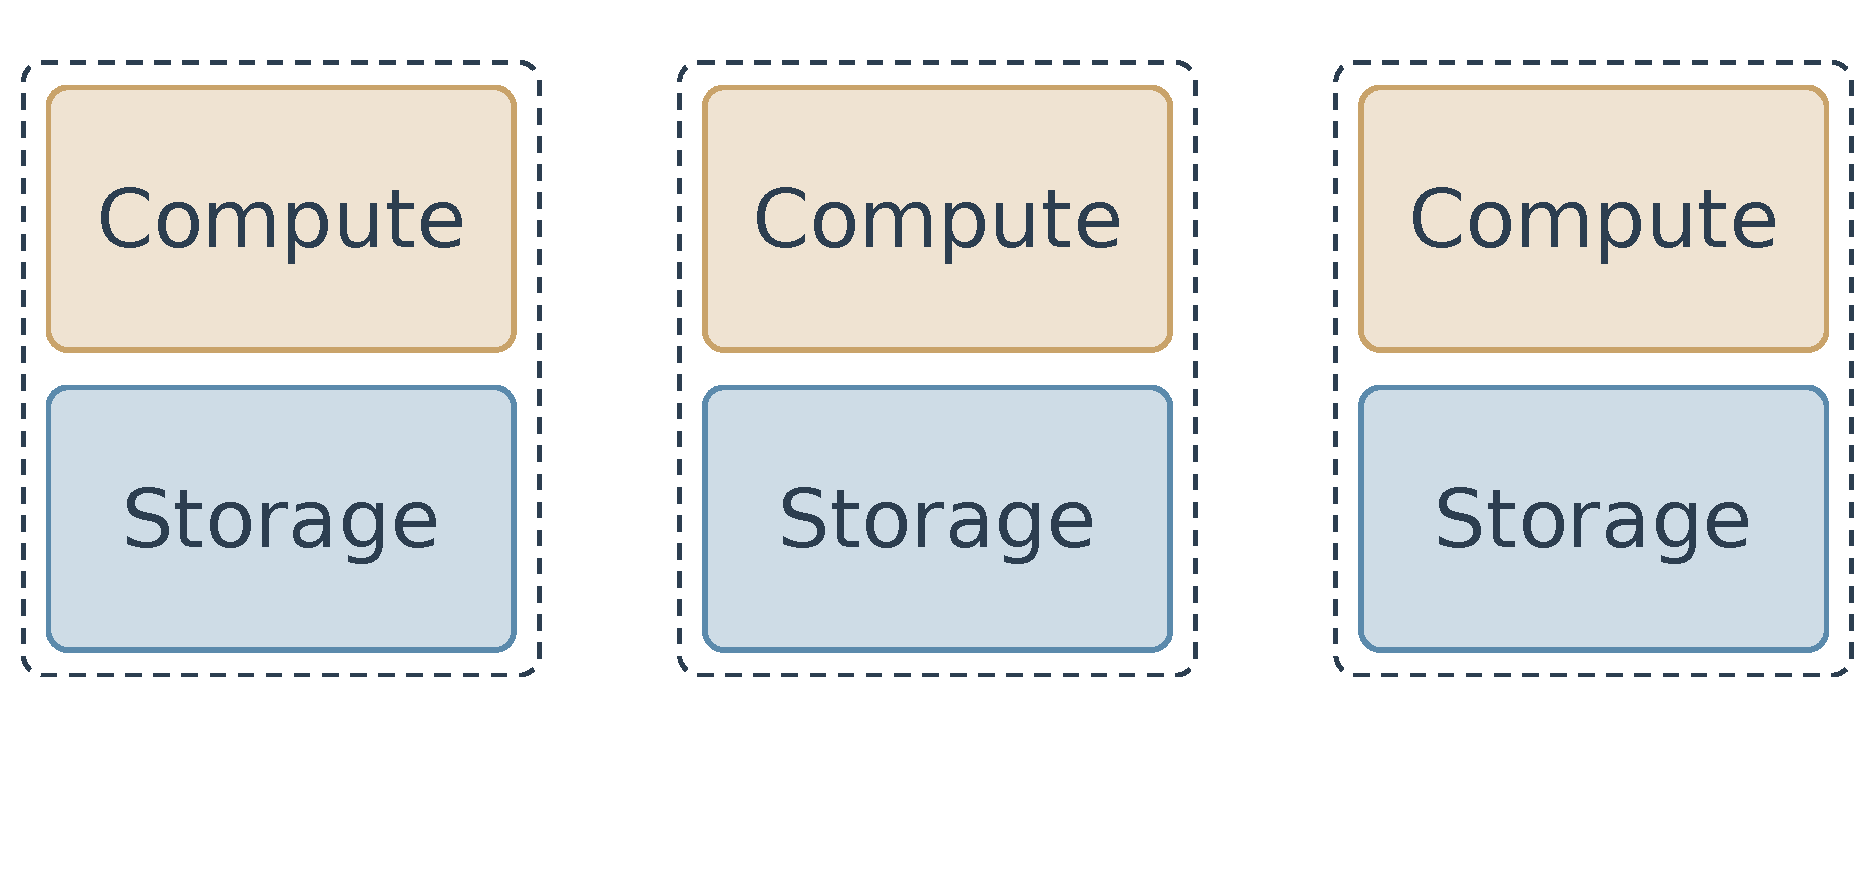
\includegraphics[valign=t, width=0.45\textwidth]{Chapters/02-background/sub-chapters/figures/02-coupled-compute.pdf}%
    }
    \hfill
    \subfloat[Decoupled storage and compute.\label{fig:decoupled-compute}]{%
        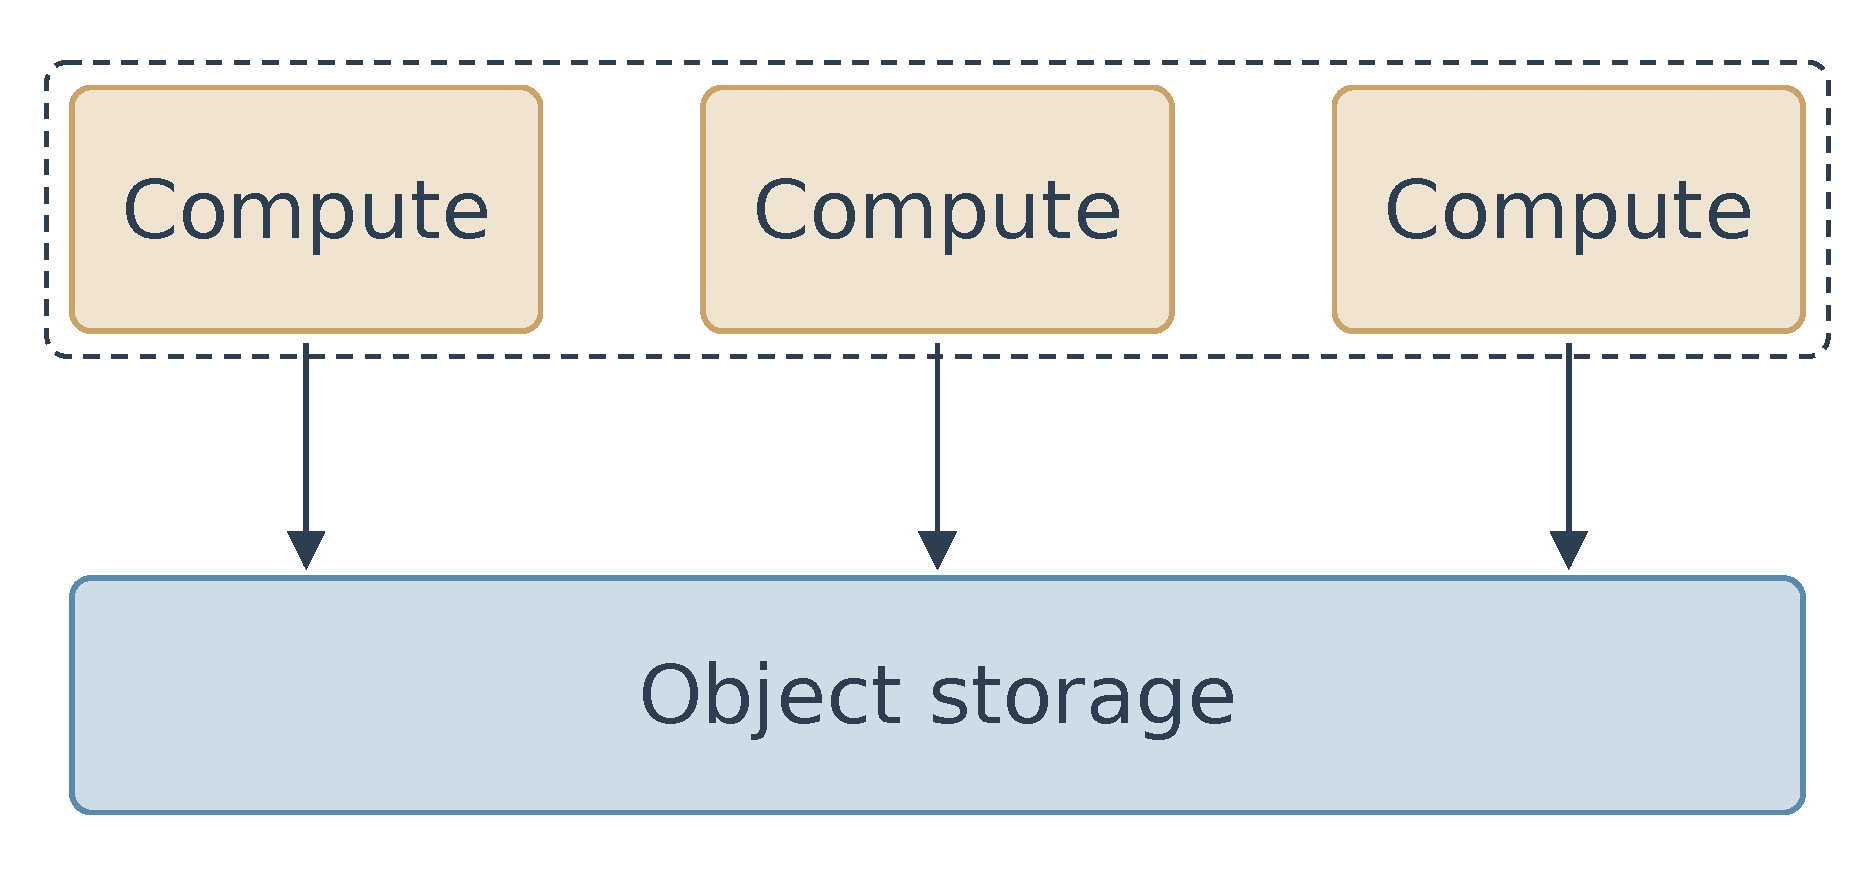
\includegraphics[valign=t, width=0.45\textwidth]{Chapters/02-background/sub-chapters/figures/02-decoupled-compute.pdf}%
    }
    \caption[Coupled versus decoupled storage and compute architectures.]{Comparison of storage and compute architectures. (a) In the traditional coupled architecture, each node bundles its own compute and storage, so the two layers must scale together as a unit. (b) In the decoupled architecture, multiple independent compute resources access a shared object storage layer, allowing storage and compute to be provisioned, priced, and scaled independently of one another.}
    \label{fig:storage-compute-architectures}
\end{figure}

\subsection{Object storage and HTTP access}
\label{background:cloud-native-data-architecture:object-storage-and-http-access}
As the shared layer underlying these architectures, object storage organizes data as opaque objects, byte sequences that the store does not inspect, each identified by a key within a flat container namespace, and serves them through a network \acrfull{api} rather than through the \acrfull{posix} file system calls used for traditional local-disk access \parencite{mesnier2003_object_based_storage, calder2011_windows_azure_storage}. Commercial implementations such as Azure Blob Storage expose each object as an \acrfull{https} \acrfull{url} accessed over \acrfull{http} \parencite{microsoft2024_azure_blob_introduction}.

Read access is mediated by \acrshort{http} itself. \textcite{fielding2022_rfc9110_http_semantics} standardize the \texttt{Range} request header, which allows a client to retrieve an arbitrary byte interval of a remote resource without downloading the whole file. Operational experience confirms the viability of this access model for analytical workloads, queries that scan and aggregate large volumes of data, at scale \parencite{vuppalapati2020_snowflake_elastic_query_engine, durner2023_exploiting_cloud_object_storage}. Cloud-native data formats are designed around this access pattern: layout metadata sits at a fixed byte offset known in advance, so that a reader fetches it first and then issues range requests for only the byte intervals required by the query \parencite{maso2023_ogc_cog_standard}, as Figure~\ref{fig:http-range-requests} illustrates.

\begin{figure}[H]
    \centering
    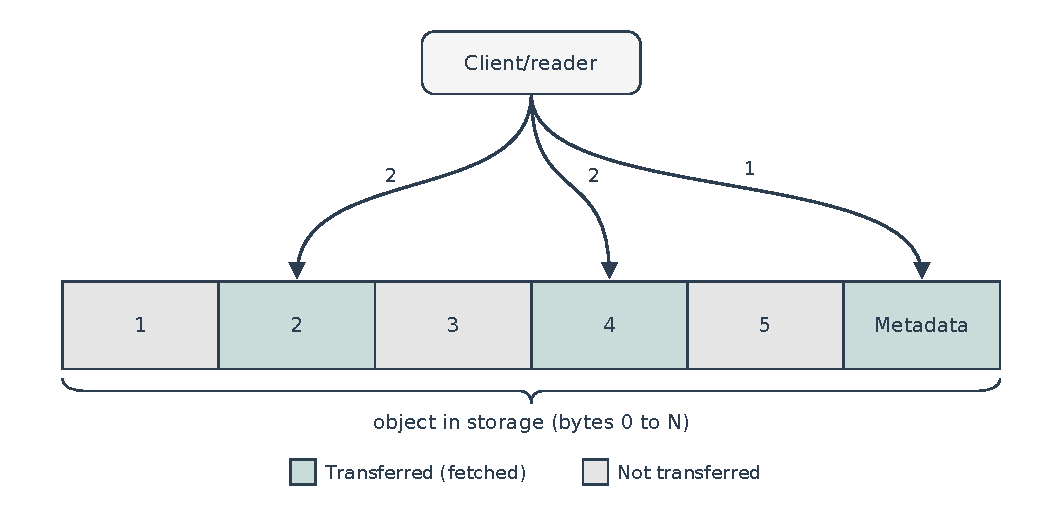
\includegraphics[width=0.85\textwidth]{Chapters/02-background/sub-chapters/figures/02-http-range-requests.pdf}
    \caption[HTTP range request access pattern.]{HTTP range request access pattern for cloud-native objects. The reader first issues a small range request for the metadata block at a known offset within the object (1), parses the layout information it returns to identify which byte intervals satisfy the query, and then issues range requests for only those intervals (2). Bytes outside the requested intervals are never transferred.}
    \label{fig:http-range-requests}
\end{figure}


\subsection{Distributed and non-distributed computation}
\label{background:cloud-native-data-architecture:distributed-and-non-distributed-computation}
With storage and compute decoupled, the choice of computational model becomes a central architectural decision. The non-distributed model runs a query end-to-end inside a single process, an operating-system execution context with its own memory, on one node, and incurs no coordination overhead between workers \parencite{mcsherry2015_scalability_but_at_what_cost}. The distributed model splits both data and computation across multiple worker nodes, where each worker handles a share of the data and runs its assigned tasks, coordinated by a driver or scheduler that dispatches work and aggregates results \parencite{stonebraker1986_case_for_shared_nothing,zaharia2012_resilient_distributed_datasets}. Figure~\ref{fig:compute-models} contrasts the two models.

\begin{figure}[H]
    \centering
    \subfloat[Non-distributed compute.\label{fig:non-distributed-compute}]{%
        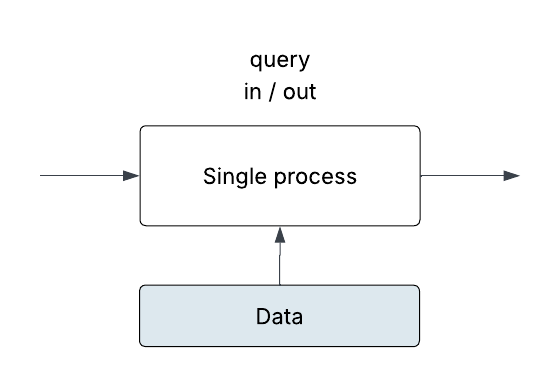
\includegraphics[valign=t, width=0.45\textwidth]{Chapters/02-background/sub-chapters/figures/02-non-distributed-compute.png}%
    }
    \hfill
    \subfloat[Distributed compute.\label{fig:distributed-compute}]{%
        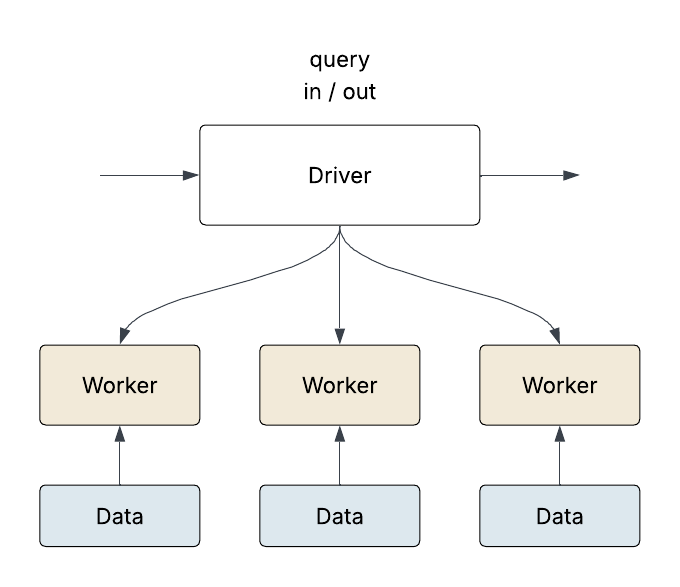
\includegraphics[valign=t, width=0.45\textwidth]{Chapters/02-background/sub-chapters/figures/02-distributed-compute.png}%
    }
    \caption[Non-distributed versus distributed compute models.]{Comparison of compute models. (a) In the non-distributed model, a single process executes the query end-to-end, with no coordination overhead between workers. (b) In the distributed model, a driver dispatches tasks to multiple workers, each operating on a partition of the data.}
    \label{fig:compute-models}
\end{figure}

This distribution introduces overhead from four sources: task scheduling, the assignment of work to specific executors; data shuffling between nodes, the network-based redistribution of intermediate data; serialization of in-memory objects into transmittable byte form; and network communication between workers. Each adds latency before any computation begins \parencite{mcsherry2015_scalability_but_at_what_cost,zaharia2012_resilient_distributed_datasets}. Distributed systems therefore outperform single-node systems only when the dataset or computation is large enough to justify the coordination cost \parencite{mcsherry2015_scalability_but_at_what_cost}. For spatial workloads in particular, the data partitioning strategy is critical: poor spatial partitioning produces skewed workloads, a recognized failure mode in which some workers process far more data than others, so the parallel efficiency, the speedup actually realized from each additional worker, degrades \parencite{tang2020_locationspark_distributed_spatial_query}.

\subsection{Cloud cost model}
\label{background:cloud-native-data-architecture:cloud-cost-model}
The choice between distributed and non-distributed compute is ultimately governed by a cost model in which every resource---storage, processing, and bandwidth---is separately metered \parencite{mell2011_nist_definition_of_cloud_computing}. Pricing follows a pay-as-you-go model: compute and storage are acquired on a short-term basis and released when no longer needed \parencite{armbrust2010_view_of_cloud_computing}. Each resource carries its own pricing dimension. Compute is billed in per-minute increments for allocated virtual cores, the processor units assigned to a workload \parencite{microsoft2024_virtual_machines_pricing}. Object storage is priced per gigabyte-month across access tiers, the storage classes that differ by retrieval frequency and per-GB cost, with transactional \acrshort{api}s, the per-request operations such as reads and writes, charged per \num{10000} operations \parencite{microsoft2024_azure_data_lake_storage_pricing}. Outbound traffic is billed per gigabyte of egress, the traffic leaving the provider's network for the public internet \parencite{microsoft2024_bandwidth_pricing}. To dampen the volatility of on-demand pricing, providers offer reserved instances, prepaid capacity commitments that lock in lower per-hour rates over one- or three-year terms \parencite{microsoft2024_azure_reservations}. Elasticity, the ability to provision and release resources rapidly to match demand \parencite{mell2011_nist_definition_of_cloud_computing}, therefore has direct cost implications: serverless platforms provision compute on a per-request basis and release it automatically when idle, so customers are charged only for active execution time, whereas long-running clusters continue to accrue charges regardless of utilization \parencite{jonas2019_berkeley_view_on_serverless_computing}.